\section{Evaluation}
\label{sec:evaluation}
This Section describes the evaluation of the proposed design.
Section \ref{sec:design} introduces the design of the experiment to evaluate the system. 
Section \ref{sec:measurements} identifies the measurements in the system for the experiment.
Section \ref{sec:experiment_data} describes the pilot test used to compute the number of replications in the actual evaluation. 
Section \ref{sec:analysis} presents the analysis of the results from the experiment. 

 
\subsection{Experiment design}
This chapter describes in detail the testing done on the prototype designed in chapter \ref{sec:middleware_architecture}, to validate its ability to fulfil the quality attributes.\\
\label{sec:design}
This experiment is supposed to test the scalability quality attribute associated with the system architecture. To test this a prototype, mainly consisting of mocked sensor data, transmits the mocked data to Kafka through a MQTT broker. The Kafka message bus creates a topic, to which a subscriber created in Spring subscribes. The subscriber transmits the data to a Postgres database, where it is stored for analysis. All of this is managed by a docker-compose network.
By using docker-compose for the different services it becomes possible to scale based on demand, which is what this experiment is testing.
The purpose of the experiment is to test if Kafka can handle increased traffic load from the publisher, which sends the data. To achieve this, several publisher services are booted up at the same time.
By testing, if Kafka can handle additional stress from the publishers, we gain insight into the system's ability to scale, if the company wants to add additional cells and therefore more sensors to the production. \\
To determine if the architecture meets the requirements set for the quality attribute a hypothesis has been formed: \\
"The architecture will be able to maintain a transmission time below 2 seconds while transmitting data from up to 20 sensors" 

\subsection{Measurements}
\label{sec:measurements}

The command “docker-compose up” is used to initiate each test.
After having the system run for 4 minutes, the publisher services are manually closed through Docker desktop.
Within the subscriber-service a REST API has been created, which exports the data from the Postgres database to JSON format.
After formatting the data to csv, it is imported to Excel ready for analysis.
The part of the data of interest is the timestamp the publisher sends, which indicates when the sensor has picked up the data, and the timestamp the Postgres database creates once it lands in the database. By subtracting the publisher timestamp from the database timestamp, we’re able to calculate the ms it takes to transmit the data from the “sensor/publisher” to the database.


\newpage
\subsection{Experiment Data}
\label{sec:experiment_data}
After running the experiments accessing the endpoint that creates a JSON file, and converting that JSON file to csv format the data was assembled into a single csv file. Figure \ref{figure:4} shows a data example of this.
\begin{figure}[!ht]
    \centering
    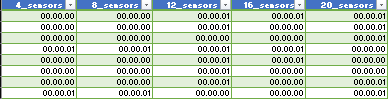
\includegraphics[scale=0.8]{Images/Data_sample.png}
    \caption{Small data sample}
    \label{figure:4}
\end{figure}

The data is stored as a time object, which goes dd(days)-hh(hours)--ss(seconds). In the example on \ref{figure:4} it can be seen that the largest transmission times hover around 1000 ms.



\subsection{Analysis}
\label{sec:analysis}
To gain an insight into all the data, each sensor's data was plotted to illustrate the differences and create a comparison.

\begin{figure}[!ht]
    \centering
    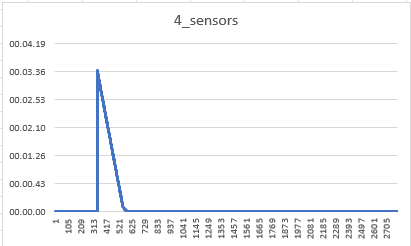
\includegraphics[scale=0.8]{Images/4sensors.png}
    \caption{4 sensors plotted}
    \label{figure:5}
\end{figure}

\begin{figure}[!ht]
    \centering
    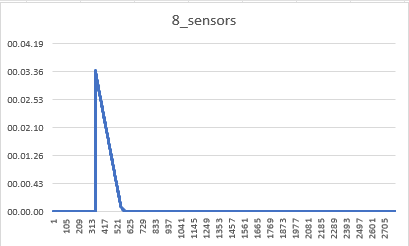
\includegraphics[scale=0.8]{Images/8sensors.png}
    \caption{8 sensors plotted}
    \label{figure:6}
\end{figure}

\begin{figure}[!ht]
    \centering
    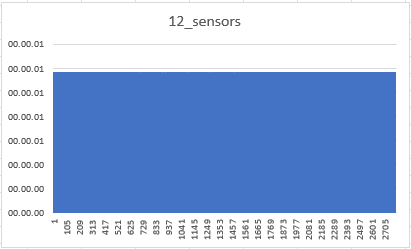
\includegraphics[scale=0.8]{Images/12sensors.png}
    \caption{12 sensors plotted}
    \label{figure:7}
\end{figure}

\begin{figure}[!ht]
    \centering
    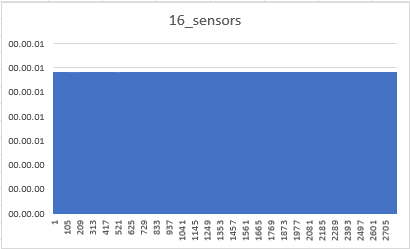
\includegraphics[scale=0.8]{Images/16sensors.png}
    \caption{16 sensors plotted}
    \label{figure:8}
\end{figure}

\begin{figure}[!ht]
    \centering
    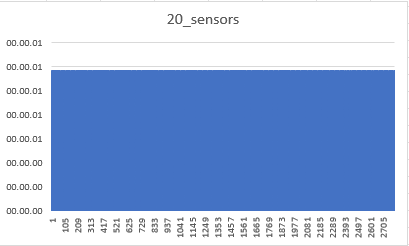
\includegraphics[scale=0.8]{Images/20sensors.png}
    \caption{20 sensors plotted}
    \label{figure:9}
\end{figure}

We can see on the graphs that sensors 4 (figure \ref{figure:5}) and 8 (figure \ref{figure:6}) tend to stay at sub 1000 ms transmission type, with similar outliers. When inspecting these outliers manually it can be seen that it is the first data sent to Kafka, which lingers until Kafka has established a connection to the database. Once the connection is established there is already live data flowing through the system, so Kafka stores the data, and sends it once the live data stream either pauses or is stopped. This results in a few outliers, matching up with the lifetime of the system during the experiment.
Once the test has 12+ sensors, the amount of data sent through the system increases, because of this, and to keep the data comparable the data was limited to 3000 samples from each test. By removing data from the past 3000 samples, the data that would have had an extended lifetime in the system from the experiments with 12, 16, and 20, does not display in the graphs.
By looking past the outliers it can be concluded that the data stays below 1s response time when scaled from 4 to 20 sensors. This means the system architecture allows scaling of producers within the system, and therefore by extension allows the addition of several cells to the system and confirms the hypothesis.